\chapter{Bewijsmethoden}\label{ch:bew:meth}
\begin{quote}
%The Final Proof of the non-Existence of God was proven by a Babel Fish.\\[2.5pt]
Now, [a Babel Fish\footnote{The Babel fish is small, yellow, leech-like - and probably the oddest thing in the universe. It feeds on brain wave energy, absorbing all unconscious frequencies and then excreting telepathically a matrix formed from the conscious frequencies and nerve signals picked up from the speech centres of the brain, the practical upshot of which is that if you stick one in your ear, you can instantly understand anything said to you in any form of language: the speech you hear decodes the brain wave matrix. \citep{adams}}] is such a bizarrely improbable coincidence that anything so mind-bogglingly useful could have evolved purely by chance that some have chosen to see it as the final proof of the NON-existence of God. The argument goes something like this:\\[2.5pt]
``I refuse to prove that I exist,'' says God, ``for proof denies faith, and without faith I am nothing.''\\[2.5pt]
``But,'' says Man, ``the Babel fish is a dead giveaway, isn't it? It could not have evolved by chance. It proves that You exist, and so therefore, by Your own arguments, You don't. QED.''\\[2.5pt]
``Oh dear,'' says God, ``I hadn't thought of that,'' and promptly vanishes in a puff of logic.\\[2.5pt]
``Oh, that was easy,'' says Man, and for an encore goes on to prove that black is white and gets himself killed on the next zebra crossing.
\end{quote}
\mbox{}\hfill\textit{Hitchhiker's Guide to the Galaxy -- \citet{adams}}\\[5pt]

{ \color{hured} Moet nog worden herzien.}

In verschillende delen van het ICT vakgebied is het wenselijk of noodzakelijk om gemaakte claims objectief en gedegen te onderbouwen, niet in de laatste plaats om anderen van de geldigheid ervan te kunnen overtuigen. Voor het geven van een onderbouwing van de geldigheid van een bewering is een heel scala van wiskundige bewijstechnieken en redeneervormen beschikbaar: \textit{bewijzen}. Voordat we deze technieken kunnen toepassen en op een generieke manier over problemen kunnen communiceren, is het in het algemeen noodzakelijk het probleem te modelleren in een formeel raamwerk: \textit{formaliseren}. Deze reader is er op gericht te oefenen met dit modelleren, en de vaardigheden op te doen in het toepassen van bewijstechnieken. 

\section{Waarom bewijzen?}
Teken eens een cirkel (of een aardappel, of iets wat daarop lijkt) met \'e\'en punt op de rand. De cirkel bestaat nu uit \'e\'en stuk. Teken nu een tweede punt op de rand, en verbind die met het eerste punt. Nu bestaat de cirkel uit twee stukken (zie ook Figuur \ref{fig:cirkel1}).
\begin{figure}
\begin{center}
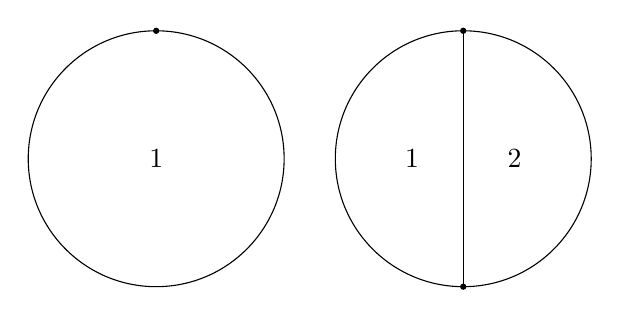
\begin{tikzpicture}[scale=.65]
\draw (3,3) circle (2.5cm);
\draw[fill=black] (3,5.5) circle (0.05cm);
\node at (3,3) {$1$};
\draw (9,3) circle (2.5cm);
\draw[fill=black] (9, 5.5) circle (0.05cm);
\draw[fill=black] (9, 0.5) circle (0.05cm);
\node at (8,3) {$1$};
\node at (10,3) {$2$};
\draw (9,5.5) -- (9,0.5);
\end{tikzpicture}
\end{center}
\caption{Cirkel met \'e\'en punt (links) en eentje met twee punten (rechts).}\label{fig:cirkel1}
\end{figure}

Teken nu een derde punt op de rand van de cirkel, en verbind die met de eerder gekozen punten. Nu bestaat de cirkel uit vier stukken. Teken ook nog een vierde punt, en verbind die weer met alle eerder gekozen punten. De cirkel bestaat nu uit acht stukken. Zie de plaatjes in Figuur \ref{fig:cirkel2}
\begin{figure}
\begin{center}
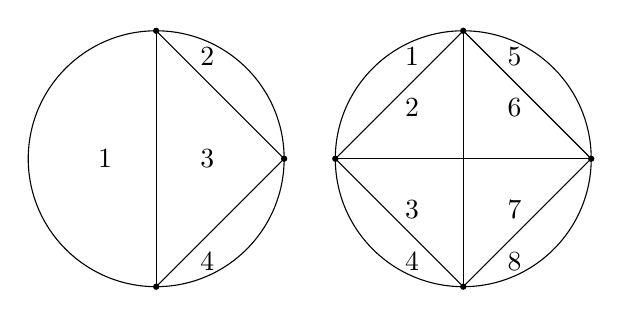
\begin{tikzpicture}[scale=.65]
\draw (3,3) circle (2.5cm);
\draw[fill=black] (3,5.5) circle (0.05cm);
\draw[fill=black] (3,0.5) circle (0.05cm);
\draw[fill=black] (5.5,3) circle (0.05cm);
\draw (3,5.5) -- (3,0.5);
\draw (3,5.5) -- (5.5,3);
\draw (5.5,3) -- (3,0.5);
\node at (2,3) {$1$};
\node at (4,5) {$2$};
\node at (4,3) {$3$};
\node at (4,1) {$4$};

\draw (9,3) circle (2.5cm);
\draw[fill=black] (9, 5.5) circle (0.05cm);
\draw[fill=black] (9, 0.5) circle (0.05cm);
\draw[fill=black] (11.5, 3) circle (0.05cm);
\draw[fill=black] (6.5, 3) circle (0.05cm);
\node at (8,1) {$4$};
\node at (8,2) {$3$};
\node at (8,4) {$2$};
\node at (8,5) {$1$};
\node at (10,1) {$8$};
\node at (10,2) {$7$};
\node at (10,4) {$6$};
\node at (10,5) {$5$};
\draw (9,5.5) -- (9,0.5);
\draw (9,5.5) -- (6.5,3);
\draw (6.5,3) -- (9,0.5);
\draw (9,0.5) -- (11.5,3);
\draw (11.5,3) -- (9,5.5);
\draw (6.5,3) -- (11.5,3);
\end{tikzpicture}
\end{center}
\caption{Cirkel met vier stukken (links); cirkel met acht stukken (rechts).}\label{fig:cirkel2}
\end{figure} 

We doen het nog een keer: we kiezen een vijfde punt en verbinden dat met de eerdere vier punten. Als we goed tellen zien we dat de cirkel nu in zestien stukken is opgedeeld. Er is hier duidelijk een patroon te zien: we beginnen met \'e\'en stuk, en elke keer als we een punt toevoegen en lijnen trekken krijgen we twee keer zo veel stukken. Bij \'e\'en punt hebben dus $2^0=1$ stukken, bij twee punten $2^1=2$, bij drie $2^2=4$ stukken, bij vier $2^3=8$ en bij vijf $2^4=16$ stukken. We concluderen nu:
\begin{quote}Als je $n$ punten op een cirkel met elkaar verbind, verdeel je daarmee de cirkel in $2^{n-1}$ stukken.\end{quote}

Dit klinkt allemaal best aannemelijk, en je bent niet zo gauw geneigd om dit nog verder uit te proberen voor zes of meer punten, want daarvoor met je toch al wel veel tekenen en tellen. Toch is het de moeite waard om dat wel eens te doen: bij zes punten lukt het je namelijk helemaal niet om $32$ stukken te krijgen, en blijft je bij $31$ stukken steken. Ook als je ervoor zorgt dat er nergens drie verbindingslijnen door \'e\'en punt gaan. We zijn er dus ingeluisd, en de hele bewering is niet waar (althans niet voor zes of meer punten).

De moraal van dit verhaal is dat als je echt zeker wilt weten dat een bewering waar is, je niet kunt vertrouwen op een paar voorbeelden en een aannemelijk verhaal dat een patroon in die voorbeelden verklaart. In de praktijk, zeker in die van de ICT, zijn er veel situaties waarin je geen genoegen kunt nemen met een paar testgevallen en een aannemelijk verhaal dat het wel goed zit. Durf je, bijvoorbeeld, te vliegen in een vliegtuig waarvan je zelf de besturingssoftware hebt geschreven, en best wel voor een redelijk aantal gevallen hebt uitgetest? Er zijn voldoende voorbeelden van dingen die fout gaan (met het verlies van mensenlevens tot gevolg) veroorzaakt door een foutje in de software \citep{fatalBugs}. Dit zijn toch dingen die je graag zou willen voorkomen.

Nu kun je niet verwachten dat je alle fouten kan voorkomen voor heel gecompliceerde dingen, maar een stap in die richting kan al heel waardevol zijn.  Wat je wilt hebben is een sluitende redenering dat een bepaalde bewering geldig is. Deze redenering kun je dan voor jezelf gebruiken, of om jezelf ervan te overtuigen dat je bewering geldig is. Maar je kunt diezelfde redenering ook gebruiken om iemand anders te overtuigen. Daarvoor is het nodig dat je de redenering opschrijft, en wel zodanig dat iemand anders aan de hand van wat je hebt opgeschreven de hele redenering ook kan volgen. En het liefst ook omgekeerd: alles wat je hebt opgeschreven speelt een essenti\"ele rol in de redenering. Zo'n redenering noemen we een \textit{bewijs}. De onderdelen van zo'n bewijs hebben een hele precieze betekenis. Een redenering met een heel precieze betekenis kun je alleen maar geven als alles wat je daarin zegt, inclusief de hele bewering waar het om gaat, heel precies is beschreven.

Vaak maak je bij het schrijven van redeneringen gebruik van manieren om je beweringen heel kort in een soort formule-taal op te schrijven, waarbij je een bijbehorende stel spelregels hebt. In dit dictaat zullen uitgebreid dergelijke notaties en begrippen aan de orde komen. Voordat we dat gaan doen lopen we eerst een aantal bewijsprincipes langs met bijbehorende voorbeelden, om een beetje een gevoel te ontwikkelen voor bewijsprincipes.

\section{Bewijzen uit het ongerijmde}\label{sec:pbc}
Bewering:
\begin{quote}
Een postbode levert $130$ poststukken af in een straat met $43$ adressen. Dan is er in die straat minstens \'e\'en adres waarop vier of meer poststukken worden afgeleverd.
\end{quote}
Hoe kun je nu het makkelijkste inzien dat deze bewering inderdaad klopt? Stel eens dat de geconcludeerde bewering (``er wordt op minstens \'e\'en adres vier of meer poststukken afgeleverd'') niet waar is. Dan worden er op elk adres dus hooguit drie poststukken afgeleverd. Met $43$ adressen in totaal betekent dat dat er in totaal hooguit $3\times 43=129$ poststukken worden afgeleverd. En dat is in tegenspraak met het gegeven dat er in totaal $130$ poststukken worden bezorgd. Dus de geconcludeerde bewering dat er minstens een adres is waarop vier of meer poststukken worden afgeleverd is wel waar, en we hebben zojuist deze bewering bewezen.

Het patroon in deze redenering komt heel vaak voor. Steeds is er een bewering waarvan je wilt bewijzen dat die waar is. De redenering zier dan als volgt uit:
\begin{quote}
Stel de bewering is niet waar. Vanuit de aanname trek je, eventueel samen met aannamen die deel uitmaken van de gegevens in de bewering, allerlei conclusies, tot je op een bewering uitkomt die niet waar is, of in tegenspraak is met gegevens in de bewering. Daaruit concludeer je dat de aanname 'de bewering is niet waar' niet kan kloppen, en daarmee is de bewering zelf wel waar.
\end{quote}

Een redenering van deze vorm wordt ook wel een bewijs uit het ongerijmde genoemd (in het Engels: proof by contradiction). In dit speciale voorbeeld wordt een telargument gegeven, dat ook wel het \textit{pigeon hole principle} (duiventilprincipe) wordt genoemd.

Als je van een bewering waarvan je denkt dat die waar is, probeert te bewijzen dat die inderdaad waar is, is het een goed idee om eens op een rijtje te zetten wat er allemaal gebeurt als die bewering niet waar is. Als het lukt om daar iets onzinnigs uit te concluderen, is de hele redenering om te vormen tot een bewijs uit het ongerijmde. 

Een waarschuwing is hier echter wel op zijn plaats: elke bewering die te bewijzen is, is op deze manier als volgt te bewijzen met een bewijs uit het ongerijmde. Stel de bewering is niet waar, geef een bewijs van de bewering, dit is in tegenspraak met de aanname dat de bewering niet waar is, en dus is de bewering waar. Wat betreft de geldigheid is hier niets tegenin te brengen, maar deze redenering bevat wel een hoop overbodige ballast: het bewijs van de bewering zelf is natuurlijk een stuk korter dan datzelfde bewijs met nog een hoop geredeneer er om heen. Uit het oogpunt van effici\"entie is een kort bewijs altijd te prefereren boven een langer bewijs. Tegen de tijd dat je een bewijs uit het ongerijmde hebt gevonden, is het dan ook altijd een goed principe om te kijken of je de redenering uit het ongerijmde wel echt nodig hebt, en niet in feite dezelfde redenering korter rechtstreeks kunt geven.

Nauw verwant aan een bewijs uit het ongerijmde is een bewijs met \textit{contrapositie}. Dat betekent dat je als een bewering van de vorm
\begin{quote}
Als $P$ geldt, dan geldt ook $Q$
\end{quote}
wilt bewijzen, in plaats hiervan ook mag bewijzen 
\begin{quote}
Als $Q$ niet geldt, dan geldt ook niet $P$.
\end{quote}

Merk op dat we twee keer het woord `niet' hebben toegevoegd, en $P$ en $Q$ hebben omgewisseld. We laten nu zien met een bewijs uit het ongerijmde dat dit nieuwe bewijsprincipe inderdaad klopt. We willen de bewering `Als $P$ geldt, dan geldt ook $Q$ bewijzen', en stellen dat dit niet  waar is. Dat  kan  alleen maar als er een  situatie bestaat waarin $P$ wel waar is, maar $Q$ niet; we  komen hier  later  uitgebreid  op  terug.  We  hadden  aangenomen dat we konden bewijzen `Als $Q$ niet geldt, dan geldt ook niet $P$'. Omdat in de  betreffende situatie $Q$ niet geldt, kunnen we dus concluderen dat dan ook $P$  niet geldt. Maar dit is in tegenspraak met de eerdere aanname dat in die situatie $P$ juist wel geldt.

Zoals gezegd is het een goed principe om van een bewering die je zou willen bewijzen, te gaan uitpluizen wat er allemaal gebeurt als die bewering niet waar is. Als het lukt om daar een tegenspraak uit af te leiden, is daarmee de bewering bewezen met een bewijs uit het ongerijmde. Als het echter niet lukt een tegenspraak te vinden, kun je juist gaan zoeken naar een voorbeeld waarvoor de bewering niet waar is. Als je zo’n voorbeeld hebt gevonden, heet dat een \textit{tegenvoorbeeld}, (Engels: \textit{counterexample}) waarmee dan juist bewezen is dat de bewering niet waar is.

\subsection{Opgaven}
\begin{exercise}[Optioneel]
Geef van elk van de volgende beweringen een bewijs of een tegenvoorbeeld:
\begin{itemize}
\item in elke groep van 50 mensen zijn er zes of meer die allemaal in dezelfde maand jarig zijn;
\item in elke groep van 50 mensen zijn er vijf of meer die allemaal in dezelfde maand jarig zijn;
\item in elke groep van 50 mensen zijn er vier of meer die allemaal in dezelfde maand jarig zijn.
\end{itemize}
\end{exercise}

\begin{exercise}[Optioneel]\label{ex:sqrt:2}
Rationale getallen zijn getallen die te schrijven zijn als $\frac{a}{b}$ voor willekeurige gehele $a$ en $b$ (d.w.z. $a,b \in \mathbb{Z}$).

Bewijs (uit het ongerijmde) dat de volgende bewering geldig is:
\begin{quote}
    Er is geen kleinste rationaal getal groter dan 0.
\end{quote}
\end{exercise}

\begin{exercise}[Optioneel]
Priemgetallen zijn natuurlijke getallen > 1 die slechts deelbaar zijn door 1 en zichzelf (bijv. 2, 3, 5, 7, 11, 13, 17, 19, 23, 29, \ldots).

Bewijs (uit het ongerijmde) dat de volgende bewering geldig is (ook wel bekend als de Stelling van Euclides):
\begin{quote}
    Er bestaat geen grootste priemgetal.
\end{quote}
\end{exercise}

\section{Bewijzen met gevalsonderscheiding}
Als je de getallen van 1 tot en met 100 bij elkaar optelt, wat komt er dan uit? Als je gaat rekenen: $1+2=3,3+3=6,6+4=10,10+5=15,\ldots$, dan ben je nog al even bezig. Het kan ook handiger:
$$1+100=101,2+99=101,3+98=101,\ldots,50+51=101$$
Nu hebben we de 100 getallen in 50 groepjes van twee opgesplitst, waarbij voor elk groepje van twee de som 101 is. Het totaal is dus $50\times 101=5050$.

Laten we het algemener bekijken (overigens ook een algemeen principe: probeer eerst een speciaal geval en als je daar iets voor verzonnen hebt, probeer dat dan algemener te maken). Als $k$ en $n$ gehele getallen zijn met $k<n$, en ik tel alle $n-k+1$ getallen van $k$ tot en met $n$ bij elkaar op, wat komt daar dan uit? Met hetzelfde trucje van zonet tellen we de eerste bij de laatste op, de op een na eerste bij de op een na laatste, en zo verder:
$$k+n=k+n,(k+1)+(n-1)=k+n,(k+2)+(n-2)=k+n,\ldots$$
Hoe eindigt dit? We zien dat het uitmaakt of het aantal $n-k+1$ even is of niet. Als dit aantal even is, krijgen we precies $\frac{n-k+1}{2}$ groepjes van twee waarvan de som steeds $k+n$ is. De som van de hele rij getallen is dus $(k+n)\times\frac{n-k+1}{2}=\frac{(k+n)(n-k+1)}{2}$.

Als het aantal oneven is, krijgen we $\frac{n-k}{2}$ groepjes van twee waarvan de som steeds $k+n$ is, en houden we het middelste element van de rij getallen over. Dat middelste getal is het gemiddelde van de eerste en de laatste, dus $\frac{k+n}{2}$. De som van al deze getallen is dus 
$$(k+n)\times\frac{n-k}{2}+\frac{k+n}{2}=\frac{(k+n)(n-k)+(k+n)}{2}=\frac{(k+n)(n-k+1)}{2}.$$
We zien dus dat ook in dit geval de som van de hele rij $\frac{(k+n)(n-k+1)}{2}$ is, en concluderen dat het in alle gevallen zo is. We hebben dus bewezen:
\begin{quote}
    Als $k$ en $n$ gehele getallen zijn met $k<n$, dan is de som van alle getallen van $k$ tot en met $n$ gelijk aan $\frac{(k+n)(n-k+1)}{2}$.
\end{quote}
In het bewijs van deze bewering hebben we een \textit{gevalsonderscheid} (Engels: \textit{case analysis}) gemaakt: voor het geval dat het aantal even was hebben we een bewijs gegeven, en voor het geval dat het aantal oneven was hebben we een ander bewijs gegeven. Aangezien elk geheel even of oneven is, hebben we hiermee voor alle gevallen een bewijs gegeven.

Net zoals bij bewijzen uit het ongerijmde is het bij bewijzen met gevalsonderscheid een goed principe om te kijken of je het gevalsonderscheid wel echt nodig hebt. Als je het namelijk niet nodig hebt, kun je waarschijnlijk een korter bewijs geven. In dit voorbeeld is dat inderdaad mogelijk als we met het maken van groepjes van twee niet stoppen als we op de helft zijn, maar nog even doorgaan:
$$k+n=k+n,(k+1)+(n-1)=k+n,(k+2)+(n-2)=k+n,\ldots$$
$$\ldots,(n-1)+(k+1)=k+n,n+k=k+n$$
Nu hebben we evenveel groepjes van twee gemaakt als het aantal getallen dat we bij elkaar op wilden tellen, namelijk $n-k+1$. Elk van deze groepjes heeft $k+n$ als som, al deze groepjes hebben dus samen $(k+n)(n-k+1)$ als som. In deze groepjes komen elk van de getallen precies twee keer voor: een keer als linkerlid van een groepje en een keer als rechterlid. Daarmee is tweemaal de gevraagde som dus gelijk aan $(k+n)(n-k+1)$, en concluderen we zonder gevalsonderscheid te maken dat de gevraagde som altijd gelijk aan $\frac{(k+n)(n-k+1)}{2}$.

In het eerste bewijs hebben we een opsplitsing in twee gevallen gemaakt: het aantal is even of het aantal is oneven. Het is ook mogelijk een probleem in meer dan twee gevallen op te splitsen. Van belang is altijd dat alle situaties die aan de voorwaarden van de bewering voldoen, onder tenminste een van de aangegeven gevallen vallen: de opsplitsing moet \textit{uitputtend} zijn, in het Engels: \textit{exhaustive}. Dat sommige situaties onder meer dan een van de gevallen vallen is niet erg. Dit illustreren we met het volgende voorbeeld:
\begin{quote}
    Voor elk re\"eel getal $x$ geldt dat $x\times x\geq 0$.
\end{quote}
We bewijzen dit als volgt: we maken het gevalsonderscheid $x\geq 0$ of $x\leq 0$. Dit onderscheid is inderdaad uitputtend: voor elk re\"eel getal $x$ geldt een van beide voorwaarden.

Als $x\geq 0$ dan is $x\times x$ het product van twee getallen die elk tenminste $0$ zijn; het product is dan ook tenminste 0.

Als $x\leq 0$ dan is $-x\geq 0$, en is $x\times x=(-x)\times(-x)$ het product van twee getallen die elk tenminste 0 zijn; het product is dan ook tenminste 0.

Voor beide gevallen hebben we nu een bewijs gegeven, en daarmee is het bewijs voltooid. Merk op dat het geval dat $x=0$ onder beide gevallen valt. In feite hebben we de bewering voor dit geval dus twee keer bewezen.

Het is een goed gebruik bij gevalsonderscheiding te beginnen bij de makkelijkste gevallen en het moeilijkste voor het laatst te bewaren.

\subsection{Opgaven}
\begin{exercise}[Optioneel]
Wat komt er uit als je alle even getallen van 2 tot en met 100 bij elkaar optelt? En wat komt er uit als je alle oneven getallen van 17 tot en met 47 bij elkaar optelt? Geeft een formule die voor elke $n$ aangeeft wat de som is van alle getallen van 2 tot en met $2n$.
\end{exercise}

\begin{exercise}[Optioneel]
Bewijs dat het kwadraat van een oneven getal altijd te schrijven is als $8n+1$ voor een geheel getal $n$.
\end{exercise}

\begin{exercise}[Optioneel]
Bewijs (met een gevalsonderscheid) de volgende stelling:
\begin{quote}
    Voor alle getallen $n\in\mathbb{Z}$ geldt $n^2 \text{ mod } 4 = 0\text{ of }1$.
\end{quote}
\end{exercise}
% We onderscheiden de volgende 2 gevallen:
% n is even: dan schrijven we n als 2m voor m ∈ Z. Nu geldt
% $n^2 = (2m)^2 = 4m^2$, en $4m^2/4 = m^2$ met rest 0.
% n is oneven: dan schrijven we n als 2m + 1 voor m ∈ Z. Nu geldt
% $n^2 = (2m + 1)^2 = 4m^2 + 4m + 1 = 4(m^2 + m) + 1$
% en $(4(m^2 + m) + 1)/4$ geeft rest 1.
% In beide gevallen hebben we rest 0 of 1.

\section{Bewijzen met inductie}
Voor beweringen die afhangen van een natuurlijk getal $n$ is het vaak handig om in het bewijs gebruik te maken van het gegeven dat de bewering voor kleinere waarden dan $n$ al waar is. Dat je daarmee toch een correct bewijs kunt leveren zegt het \textit{principe van volledige inductie}. In hoofdstuk \ref{ch:inductie} zal dit uitgebreid aan de orde komen.

\section{Bewijzen met invarianten}
\begin{remark}
De stof in deze sectie behoort niet tot de basisstof van het vak en zal niet getentamineerd worden. Ze is enkel toegevoegd voor ge\"interesseerde studenten die \textit{verder} willen dan de gemiddelde student.
\end{remark}
Alvorens het principe uit te leggen beginnen we met een aantal puzzels.

\subsection*{De keukenvloer}
We hebben een vierkante keukenvloer met een zijde van $n$ decimeter. In de rechteronderhoek en in de linkerbovenhoek mist een vierkante decimeter (voor een verwarmingsbuis). Voor welke $n$ kan de keukenvloer met tegels van $2\times 1$ decimeter betegeld worden? Bijvoorbeeld voor $n=6$ is de situatie als volgt:
\begin{center}
    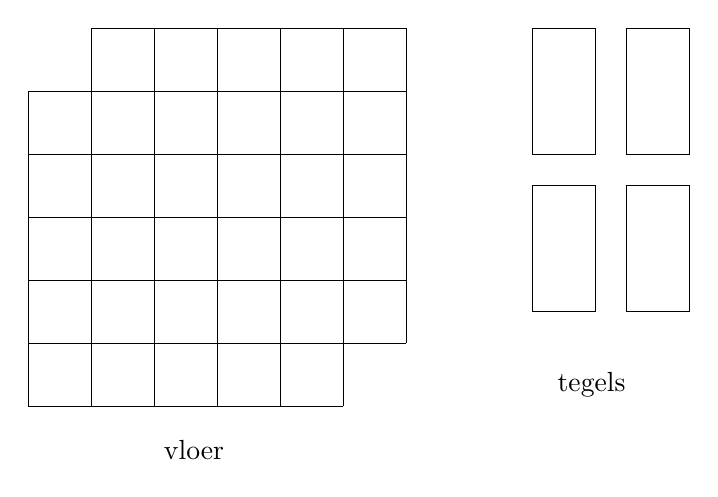
\begin{tikzpicture}[scale=.8]
    \draw[thin] (0,0) grid (5,5);
    \draw[thin] (-1,-1) grid (4,4);
    
    \draw[thin] (7, 0.5) rectangle (8,2.5);
    \draw[thin] (8.5, 0.5) rectangle (9.5, 2.5);
    \draw[thin] (7, 3) rectangle (8,5);
    \draw[thin] (8.5, 3) rectangle (9.5, 5);
    
    \node[anchor=south west] at (1,-2) {vloer};
    \node[anchor=south west] at (7.25, -1) {tegels};
    \end{tikzpicture}
\end{center}

\subsection*{De koffiekan}
In een koffiekan zitten 25 zwarte en 25 witte bonen. De volgende handeling wordt uitgevoerd zolang dat mogelijk is: \textit{haal twee bonen uit de kan; als ze dezelfde kleur hebben, stop dan een zwarte boon in de kan; als ze verschillend van kleur zijn, stop dan de witte boon terug in de kan}. Er is voldoende voorraad extra zwarte bonen. Vraag: wat is de kleur van de laatste boon in de kan?

\subsection*{De oplossingen}
Deze puzzels zijn allemaal gebaseerd op herhaling: herhaald tegels leggen en herhaald bonen trekken. Ze kunnen opgelost worden door steeds een geschikte \textit{invariant} te beschouwen, een eigenschap die steeds blijft gelden. We geven eerst de definitie.

\begin{definition}[Invariant]\mbox{}\\
Een invariant is een eigenschap van een proces of programma, die voldoet aan het volgende:
\begin{itemize}
    \item aan het begin geldt de invariant, en
    \item als de invariant geldt en er wordt vervolgens een stap gedaan, dan geldt na afloop van die stap de invariant weer.
\end{itemize}
\end{definition}

Als we zo'n eigenschap hebben, blijft die dus altijd gelden, hoeveel stappen er ook worden uitgevoerd. Als na eindig veel stappen het proces of programma voltooid is, geldt de invariant na afloop dus nog steeds. Deze observatie is cruciaal voor de oplossingen van elk van de puzzels, en is een belangrijk bewijsprincipe in de informatica.

\subsection*{Oplossing voor de keukenvloer}
We maken een gevalsonderscheid. Als $n$ oneven is dan is $n^2$ oneven, en $n^2-2$ dus ook. Een vloer van een oneven aantal dm$^2$ is nooit te betegelen met tegels die elk $2$ dm$^2$ groot zijn.

Als $n$ even is dan kleuren we de vloer in gedachten als een schaakbord: om en om wit en zwart, met de rechteronderhoek wit. De twee verwarmingsbuizen staan in een wit veld. Er moeten dus twee zwarte velden m\'e\'er betegeld worden dan witte velden. Omdat elke tegel \'e\'en zwart en \'e\'en wit veld bedekt, zullen we, hoe we ook tegelen, altijd twee zwarte velden overhouden. Een betegeling is dus niet mogelijk.

We hebben gebruik gemaakt van de invariant
$$\text{\it aantal onbetegelde zwarte velden = aantal onbetegelde witte velden + 2}$$
Deze uitspraak is in het begin waar, en blijft invariant bij het leggen van een tegel. De uitspraak geldt dus voor alle gedeeltelijke betegelingen, en er is geen betegeling waarin geen onbetegelde zwarte velden over zijn.

\subsection*{Oplossing voor de koffiekan}
Allereerst merken we op dat bij elke trekking er twee bonen verwijderd worden, en \'e\'en teruggelegd. Na 49 trekkingen zal er dus nog \'e\'en boon over zijn.

Het is ondoenlijk om alle mogelijkheden te proberen, dat zijn er heel erg veel. In plaats daarvan zoeken we naar een geschikte invariant. We kijken naar het netto effect op het aantal witte en zwarte bonen bij elk van de vier mogelijke trekkingen:
\begin{center}
    \begin{tabular}{|cc|cc|}
    \hline
    trekking & actie & $Z$ & $W$ \\
    \hline
    $-ZZ$ & $+Z$ & -1 & 0\\
    $-WW$ & $+Z$ & +1 & -2\\
    $-ZW$ & $+W$ & -1 & 0\\
    $-WZ$ & $+W$ & -1 & 0\\
    \hline
    \end{tabular}
\end{center}
Het witte aantal bonen in de kan blijft gelijk of neemt met twee af. Het oneven-zijn van het aantal witte is dus een invariant in dit spel!

Het aantal witte bonen blijft dus altijd oneven, in het bijzonder aan het eind. De laatste is dus altijd wit.

\subsection{Opgave}
\begin{exercise}[Optioneel]
In een doos zitten 100 rode, 100 witte en 100 blauwe ballen. Zolang dat mogelijk is, worden er drie ballen uit de doos gepakt. Als alle drie de ballen dezelfde kleur hebben, wordt er \'e\'en van die drie teruggelegd. Als alle drie de ballen een verschillende kleur hebben, wordt een rode bal teruggelegd. Als er twee ballen dezelfde kleur hebben, wordt de afwijkende derde teruggelegd en bovendien een blauwe. Is het mogelijk te eindigen met een rode en een blauwe bal?
\end{exercise}

\begin{exercise}[Optioneel]
Met de volgende regels kun je van rijtjes symbolen andere rijtjes symbolen maken:
\begin{enumerate}[label=\arabic*.]
    \item achter een rijtje met een $\mathsf{I}$ mag je een $\mathsf{U}$ zetten;
    \item van een rijtje $\mathsf{M}x$ mag je $\mathsf{M}xx$ maken, voor elk rijtje symbolen $x$;
    \item als er $\mathsf{I}\mathsf{I}\mathsf{I}$ in een rijtje staat, dan mag je dat vervangen door $\mathsf{U}$
    \item als er $\mathsf{U}\mathsf{U}$ in een rijtje staat, mag je dat weglaten.
\end{enumerate}
Als voorbeeld bekijken we een aantal rijtjes die je uit $\mathsf{MI}$ kunt produceren:

\begin{tabular}{lll}
a. & $\mathsf{MI}$ & gegeven \\
b. & $\mathsf{MII}$ & uit a volgens regel 2 \\
c. & $\mathsf{MIIII}$ & uit b volgens regel 2 \\
d. & $\mathsf{MIIIIU}$ & uit c volgens regel 1 \\
e. & $\mathsf{MUIU}$ & uit d volgens regel 3 \\
f. & $\mathsf{MUIUUIU}$ & uit e volgens regel 2 \\
g. & $\mathsf{MUIIU}$ & uit f volgens regel 4 
\end{tabular}

\noindent
Vraag: is het mogelijk om beginnend met het rijtje $\mathsf{MI}$ uit te komen op het rijtje $\mathsf{MU}$? Zo ja, hoe? Zo nee, waarom niet?\\
(Aanwijzing: laat zien dat in geen enkel opgebouwd rijtje het aantal $\mathsf{I}$'s een drievoud is.)
\end{exercise}
